\lecture{异常处理}{lec:chap10}
\section[异常]{异常}\label{sec:chap10-sec01}
%%%%%%%%%%%%%%%%%%%%%%%%%%%%%%%%%%%%%%%%
\begin{frame}[t, fragile]{异常}{简介}%
  \stretchon
  \begin{itemize}
  \item 错误:语法错误,逻辑错误和运行错误。
  \item 常见异常错误:数组下标越界、运算溢出、除0、动态分配内存失败和
    文件读写失败。
  \item 异常处理机制:\cppinline{try-throw-catch}
  \end{itemize}
  \stretchoff
\end{frame}
%%%%%%%%%%%%%%%%%%%%%%%%%%%%%%%%%%%%%%%%

\section[try块]{try块}\label{sec:chap10-sec02}
%%%%%%%%%%%%%%%%%%%%%%%%%%%%%%%%%%%%%%%%
\begin{frame}[t, fragile]{try块}{try块}%
  \stretchon
  \begin{itemize}
  \item 能够抛出异常的语句被包围在try块中。
  \item try块以关键字try 开始,后面是花括号括起来的语句序列。try块之后
    紧跟一组处理代码,称为catch子句。try块将语句分成组,并将它们与处理
    这些语句可能抛出的异常的语句相关联。    
  \end{itemize}
  \stretchoff
\end{frame}
%%%%%%%%%%%%%%%%%%%%%%%%%%%%%%%%%%%%%%%%

\section[catch块]{catch块}\label{sec:chap10-sec03}
%%%%%%%%%%%%%%%%%%%%%%%%%%%%%%%%%%%%%%%%
\begin{frame}[t, fragile]{catch块}{catch块}%
  \begin{itemize}
  \item C++的异常处理代码是catch子句。当一个异常被try块中的语句抛出时,
    系统在try块后的catch子句列表中查找能够处理该异常的catch子句。    
  \end{itemize}  
\end{frame}
%%%%%%%%%%%%%%%%%%%%%%%%%%%%%%%%%%%%%%%%

\section[示例]{异常处理示例}\label{sec:chap10-sec04}
%%%%%%%%%%%%%%%%%%%%%%%%%%%%%%%%%%%%%%%%
\begin{frame}[t, fragile]{示例}{实例分析}%
  \begin{itemize}
  \item 一元二次方程的根
  \end{itemize}
  \begin{center}
    \begin{tikzpicture}[font=\tiny, show background grid]
      \tikzset{coord/.style={coordinate}}
      \umlnote[scale=0.7, text width=0.6\textwidth] (code1) at (0, 0)
      {
        \cppfilenobg{codes/chap10/testTryCatch01/01-structdef.cpp}
      };
    \end{tikzpicture}
  \end{center}
\end{frame}

\begin{frame}[t, fragile]{示例}{实例分析}%
  \begin{itemize}
  \item 一元二次方程的根
  \end{itemize}
  \begin{center}
    \begin{tikzpicture}[font=\tiny, show background grid]
      \tikzset{coord/.style={coordinate}}
      \umlnote[scale=0.9, text width=0.7\textwidth] (code1) at (0, 0)
      {
        \cppfilenobg{codes/chap10/testTryCatch01/02-mainfun.cpp}
      };
    \end{tikzpicture}
  \end{center}
\end{frame}
\section[文件异常]{文件异常}\label{sec:chap10-sec05}
%%%%%%%%%%%%%%%%%%%%%%%%%%%%%%%%%%%%%%%%
\begin{frame}[t, fragile]{文件异常}{文件异常}%
  \begin{itemize}
  \item 文件异常
  \end{itemize}
  \begin{center}
    \begin{tikzpicture}[font=\tiny, show background grid]
      \tikzset{coord/.style={coordinate}}
      \umlnote[scale=1.0, text width=0.65\textwidth] (code1) at (0, 0)
      {
        \cppfilenobg{codes/chap10/testfileexception/main.cpp}
      };
    \end{tikzpicture}
  \end{center}
\end{frame}
%%%%%%%%%%%%%%%%%%%%%%%%%%%%%%%%%%%%%%%%

\section[预定义异常]{系统预定义异常}\label{sec:chap10-sec06}
%%%%%%%%%%%%%%%%%%%%%%%%%%%%%%%%%%%%%%%%
\begin{frame}[t, fragile]{预定义异常}{系统预定义异常}%
  \begin{itemize}
  \item 系统预定义异常
  \end{itemize}
  \begin{center}
    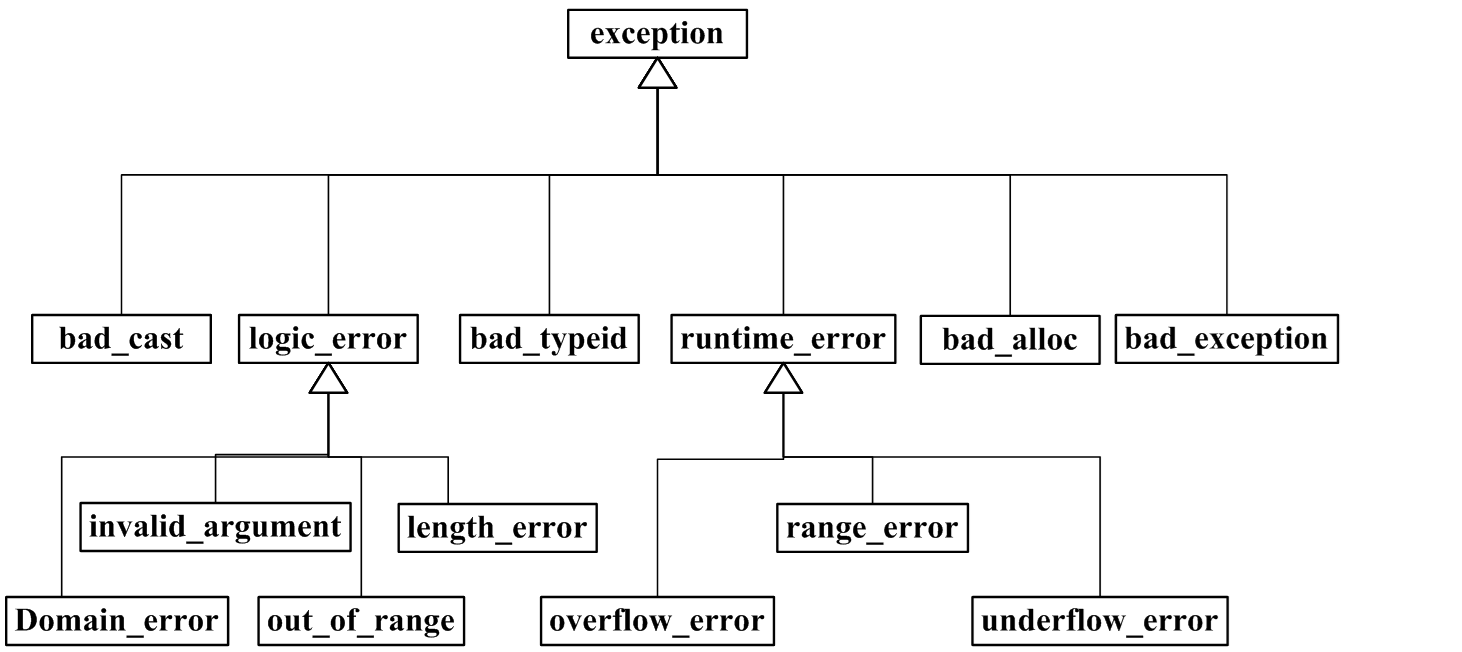
\includegraphics[width=0.95\textwidth]{figure/chap10/01trycatchclass}
  \end{center}
\end{frame}
%%%%%%%%%%%%%%%%%%%%%%%%%%%%%%%%%%%%%%%%

\section[异常的使用]{异常的使用}\label{sec:chap10-sec07}
%%%%%%%%%%%%%%%%%%%%%%%%%%%%%%%%%%%%%%%%
\begin{frame}[t, fragile]{异常的使用}{异常的使用}%
  \stretchon
  \begin{itemize}
  \item 集中处理容易出问题的代码。
  \item 异常只是错误处理技术的一种,程序中还应该使用其他错误处理技术,
    如断言、返回错误代码等。
  \item 异常使程序的复杂性增加,可以参考一些指导原则,慎用异常机制。
  \end{itemize}
  \stretchoff
\end{frame}
%%%%%%%%%%%%%%%%%%%%%%%%%%%%%%%%%%%%%%%%
% 附件页
\section[附件下载]{本讲示例代码及附件下载} 
\begin{frame}{附件}{本讲附件}
  % 此处的[ucfilespec=...]必须指定为pdf否则Windows下无法下载
  %\vspace{-4ex}
  \textattachfile[ucfilespec=ex-src10.pdf]{ex-src10.zip}{附件:右键单击该
    链接,选择\qtmark{\alert{保存附件}}下载,\alert{将后缀名改为\qtmark{.zip}解压}
      \footnote[frame]{请\alert{退出全屏模式}后点击该链接。}
      \footnote[frame]{以Adobe Acrobat Reader为例。}
      。}%\\

  \vspace{-1ex}
  \begin{center}
    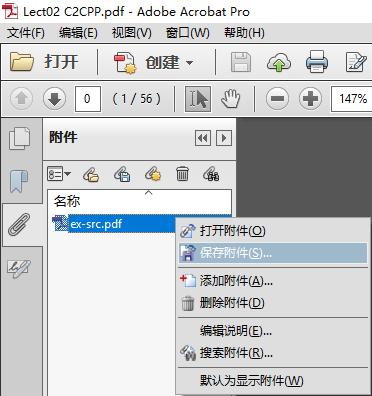
\includegraphics[height=0.35\textheight]{pdfattatchdownload01}\quad
    %或 \quad%
    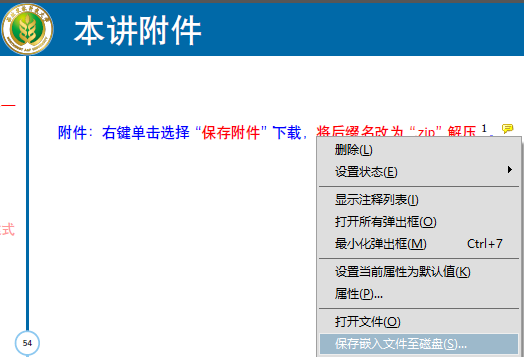
\includegraphics[height=0.35\textheight]{pdfattatchdownload02}\\[2ex]%
    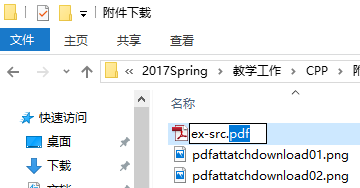
\includegraphics[height=0.255\textheight]{pdfattatchdownload03}\quad
    %$\Rightarrow$ \quad%
    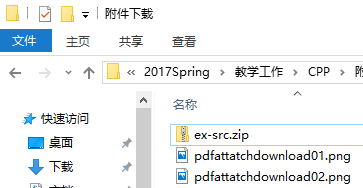
\includegraphics[height=0.255\textheight]{pdfattatchdownload04}%
  \end{center}   
\end{frame}


% \tiny
% \scriptsize
% \footnotesize
% \small
% \normalsize
% \large
% \Large
% \LARGE
% \huge
% \Huge


%%% Local Variables: 
%%% mode: latex
%%% TeX-master: "../main.tex"
%%% End: 
